\chapter*{Ça commence : vers l’île de Chiloe\markboth{Ça commence : vers l’île de Chiloe}{}}
\section*{13 février 2015}
Arrivée à Santiago du Chili avec la mauvaise surprise de voir le carton du vélo ouvert et une pédale manquante. Je demande au personnel des bagages s'ils peuvent la retrouver mais sans succès. 

 Au passage c'était une bonne idée d'apprendre un peu d'espagnol parce que quasiment personne ne parle anglais, même à l'aéroport.
\begin{center} 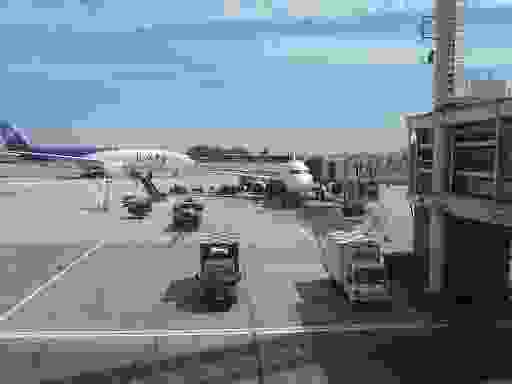
\includegraphics[width=\mywidth]{../wp-content/uploads/2015/02/P2092025.jpg} \end{center}

 Dernier vol entre Santiago et Puerto Montt : je cherche un moyen pour rejoindre le centre ville comme je ne peux pas monter le vélo. 
 Pas de chance le seul distributeur de l'aéroport est vide et les CB ne sont pas acceptées pour le bus ou les taxis. 
Heureusement une touriste allemande me propose de partager un taxi. Et au moment de charger le vélo dans le taxi, la pédale que je croyais perdue tombe du carton, ouf ! 

 Le taxi nous pose à l'hôtel de l'allemande et je vois que la personne chez qui je devais rester en couchsurfing ne peut pas m'accueillir finalement. Du coup je reste à l'hôtel pour cette première nuit.
\begin{center} 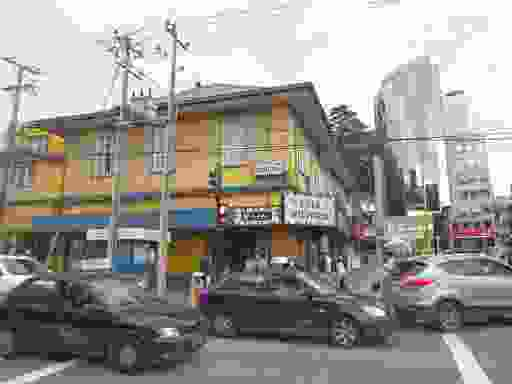
\includegraphics[width=\mywidthreduced]{../wp-content/uploads/2015/02/P2092027.jpg} \end{center}

 Puerto Montt, le bord de mer.
\begin{center} 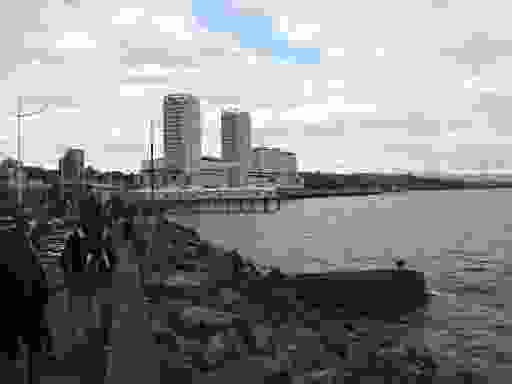
\includegraphics[width=\mywidthreduced]{../wp-content/uploads/2015/02/P2092029.jpg} \end{center}

 Le lendemain, 60 km d'autoroute vers l'île de Chiloe.
\begin{center} 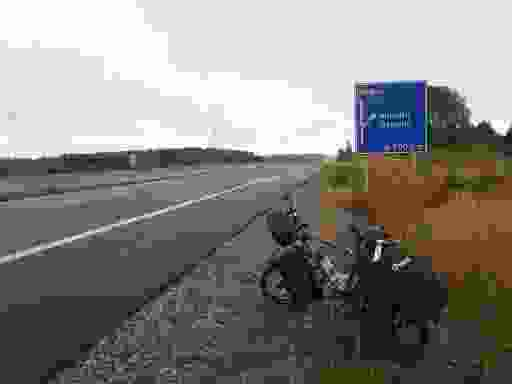
\includegraphics[width=\mywidth]{../wp-content/uploads/2015/02/P2102037.jpg} \end{center}

 Puis traversée en ferry.
\begin{center} 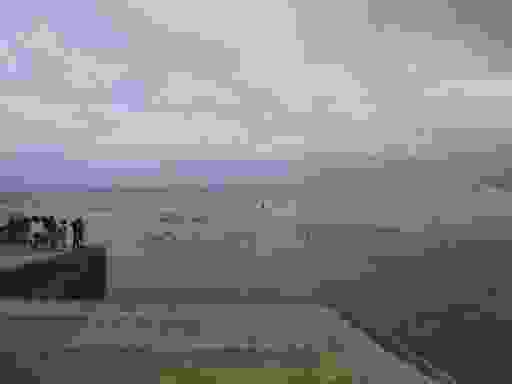
\includegraphics[width=\mywidth]{../wp-content/uploads/2015/02/P2102039.jpg} \end{center}
\vspace{-\topsep}

\pagebreak
~
\begin{center} 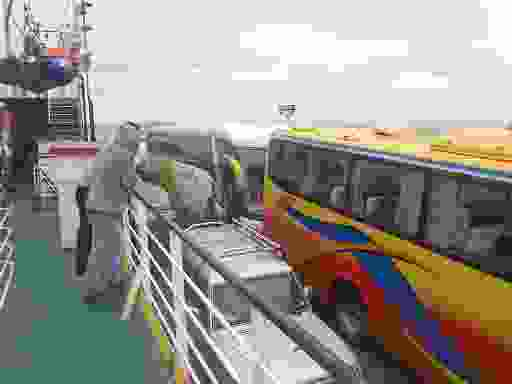
\includegraphics[width=\mywidth]{../wp-content/uploads/2015/02/P2102041.jpg} \end{center}
~
\begin{center} 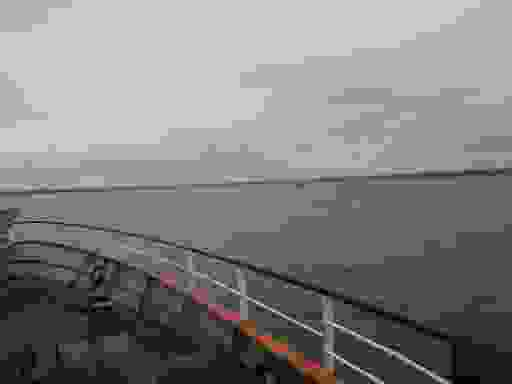
\includegraphics[width=\mywidth]{../wp-content/uploads/2015/02/P2102043.jpg} \end{center}
\vspace{-\topsep}

\pagebreak
 Petit village de Chacao.\\
\begin{center} 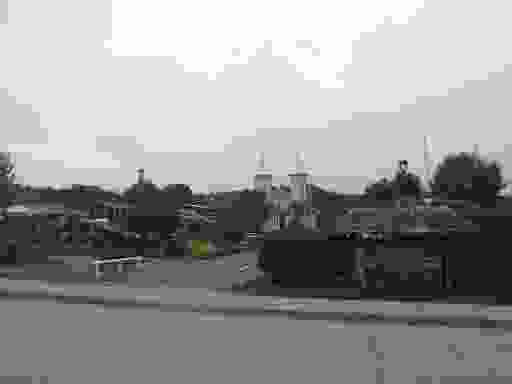
\includegraphics[width=\mywidth]{../wp-content/uploads/2015/02/P2102045.jpg} \end{center}
~\\

~
\begin{center} 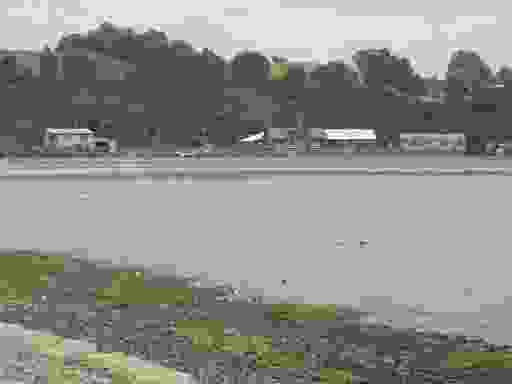
\includegraphics[width=\mywidth]{../wp-content/uploads/2015/02/P2102047.jpg} \end{center}
\vspace{-\topsep}

\pagebreak
 Première nuit de camping, pas simple de trouver un endroit car presque tout est clôturé sur l'île, j'ai du demander pour m'installer. 
\begin{center} 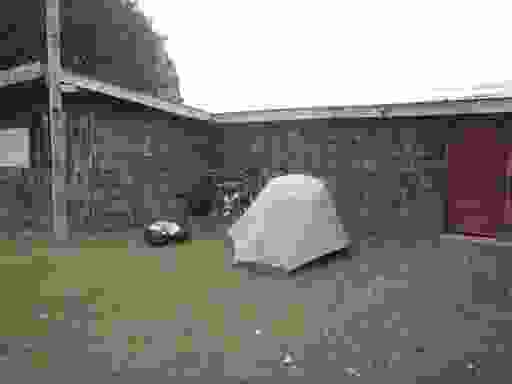
\includegraphics[width=\mywidth]{../wp-content/uploads/2015/02/P2112048.jpg} \end{center}

 25km de route vers la ville d'Ancud où je rencontre 3 cyclistes, 2 français et 1 espagnol, l'occasion de recevoir quelques conseils.

 Le port d'Ancud.
\begin{center} 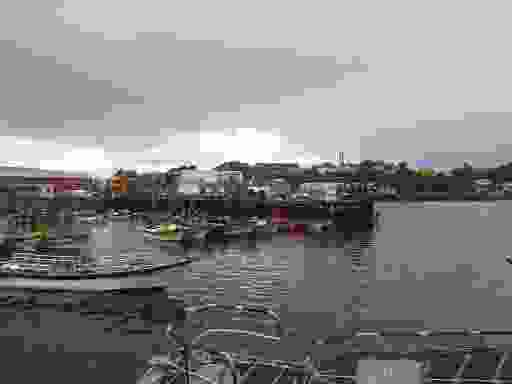
\includegraphics[width=\mywidth]{../wp-content/uploads/2015/02/P2122061.jpg} \end{center}
\vspace{-\topsep}

\pagebreak
~
\vspace{-3mm}
\begin{center} 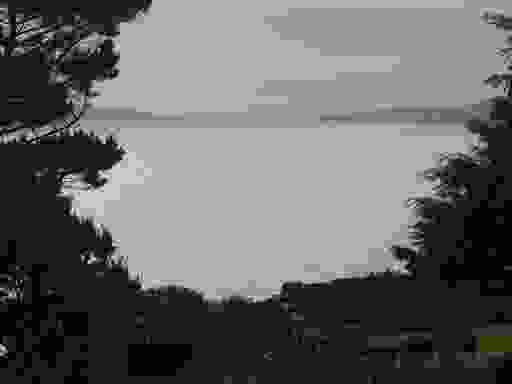
\includegraphics[width=\mywidth]{../wp-content/uploads/2015/02/P2122063.jpg} \end{center}

 Camping avec douche chaude.
\begin{center} 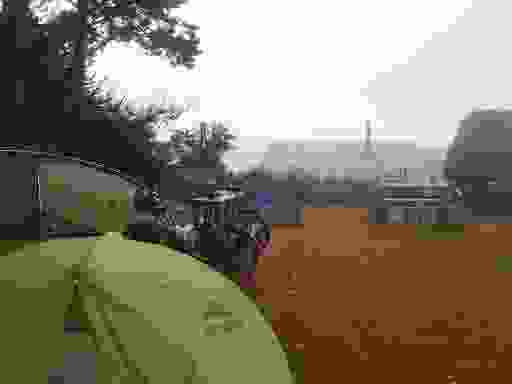
\includegraphics[width=\mywidth]{../wp-content/uploads/2015/02/P2122057.jpg} \end{center}
\vspace{-\topsep}

\pagebreak
Spécialité chilienne : pomme de terre frite avec une garniture viande / olives.
\begin{center} 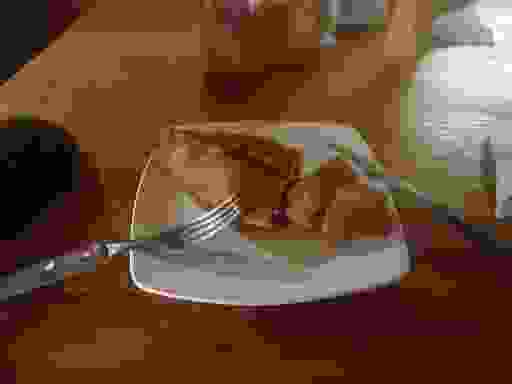
\includegraphics[width=\mywidth]{../wp-content/uploads/2015/02/P2122060.jpg} \end{center}
